\documentclass[border=1pt]{standalone}
\usepackage[dvipsnames]{xcolor}
\usepackage{tikz}                       % Graphen und kommutative Diagramme
\usetikzlibrary{patterns}               % Um schraffierte Formen in der tikzpicture-Umgebung zu zeichnen.
\newcommand{\ul}[1]{\underline{\smash{#1}}}

\begin{document}
\centering
\begin{minipage}{.35\textwidth}
\centering
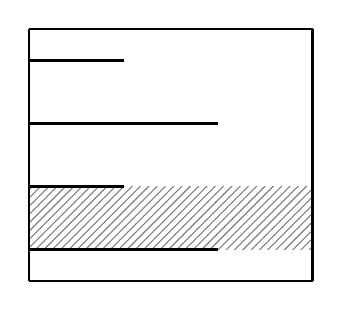
\begin{tikzpicture}[yscale=.8, xscale=1.2, line width=1pt]
    \filldraw[pattern=north east lines, pattern color=gray, draw=none] (0, 1) -- (3, 1) -- (3,2) -- (0,2) -- cycle;
    
    \draw (0,0.5) -- (3,0.5);
    \draw (0,4.5) -- (3,4.5);
    \draw (0,0.5) -- (0,4.5);
    \draw (3,0.5) -- (3,4.5);
    
    \draw[line width=1pt] (0,4) to (1,4);
    \draw[line width=1pt] (0,2) to (1,2);
    
    \draw[line width=1pt] (0,3) to (2,3);
    \draw[line width=1pt] (0,1) to (2,1);
\end{tikzpicture}
\end{minipage}
\hspace{.7cm}
\begin{minipage}{.35\textwidth}
\centering
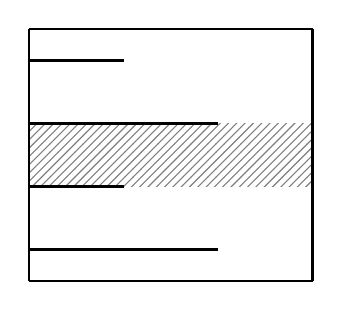
\begin{tikzpicture}[yscale=.8, xscale=1.2, line width=1pt]
    \filldraw[pattern=north east lines, pattern color=gray, draw=none] (0, 2) -- (3, 2) -- (3,3) -- (0,3) -- cycle;
    
    \draw (0,0.5) -- (3,0.5);
    \draw (0,4.5) -- (3,4.5);
    \draw (0,0.5) -- (0,4.5);
    \draw (3,0.5) -- (3,4.5);
    
    \draw[line width=1pt] (0,4) to (1,4);
    \draw[line width=1pt] (0,2) to (1,2);
    
    \draw[line width=1pt] (0,3) to (2,3);
    \draw[line width=1pt] (0,1) to (2,1);
\end{tikzpicture}
\end{minipage}
\end{document}